\chapter{Krunimír: želví grafika}
\label{chap:krunimir}

\begin{quotation}
Želvák Krunimír je velký myslitel. Zjistil, ze když si za krunýř přiváže trochu
křídy, kreslí za sebou při svém plazení cestičku. I pojal plán nakreslit svoji
podobiznu, samozřejmě včetně přesných detailů krunýře. Hned se dal pln nadšení
do díla a práce mu šla pěkně od ... tlapy.

\uv{Co to děláš, dědečku,} zeptal se jednou Krunimíra jeho vnuk Krunoslav.
\uv{Krešlím tady švou poďobižnu,} odpověděl Krunimír. \uv{Žačal jsem š ní, když
tvůj tatík ještě nebyl na švětě, a ještě nemám ani krunýř,} dodal smutně. \uv{To
už ji aši dokrešlit neštihnu...}  Vnuk Krunoslav, znalec moderní techniky, mu
však poradil: \uv{Tak si nech napsat program, který ji nakreslí za Tebe.}
Protože se ale s tlapami a zobákem moc dobře neprogramuje, najali si želváci
vás.
\end{quotation}

Takto začíná zadání finální úlohy Soutěže v programování z roku
2010 \cite{krunimir-task} (přetisknuto na straně \pageref{pdf:krunimir}).
Popisuje jednoduchý procedurální jazyk na generování želví grafiky, inspirovaný
jazykem Logo, a úkolem je vytvořit interpret tohoto jazyka, jehož vstupem je
text programu a výstupem vykreslený obrázek. 

\begin{figure}
  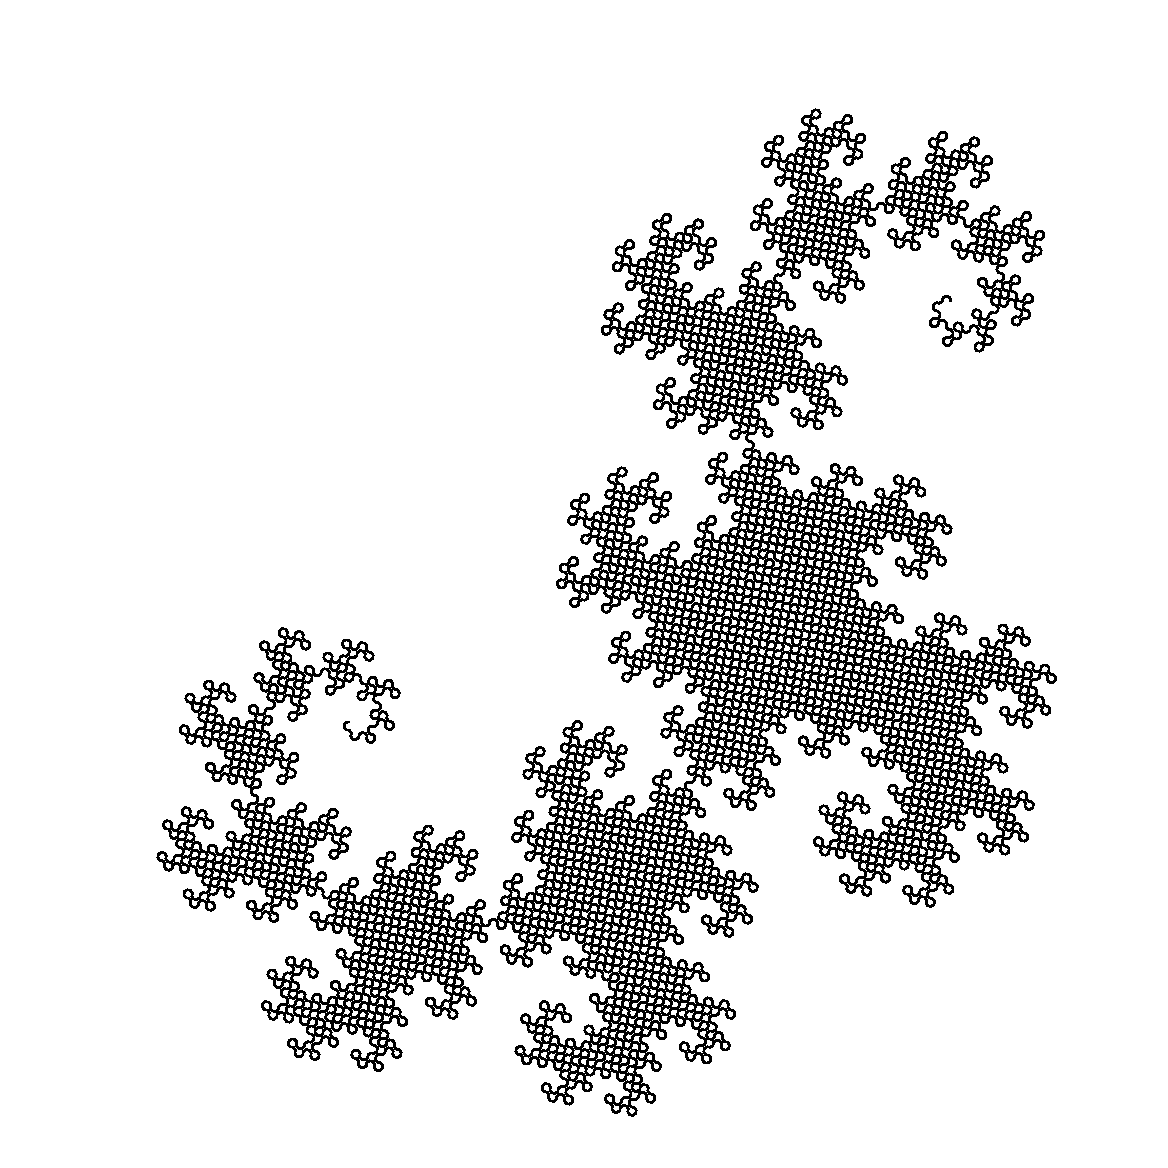
\includegraphics[width=0.9\textwidth]{krunimir/examples/dragon}

  \caption{Příklad obrázku vykresleného pomocí Krunimírova jazyka (Dračí
  křivka)}
  \label{fig:krunimir-dragon}
\end{figure}

\section{Popis jazyka}

Krunimírův jazyk umožňuje vykreslovat obrázky principem želví grafiky. Na
začátku se želva nachází uprostřed obrázku o velikosti 701\texttimes701 pixelů
vyplněného bílou barvou a je otočená směrem nahoru. Uživatel má k dispozici
několik primitivních kreslících procedur, kterými může želvu ovládat:

\begin{description}

\item[@t{forward(d)}] Želva se posune vpřed o @t{d} jednotek (pixelů).  Pokud je
  tloušťka pera kladná, zanechá za sebou čáru vedoucí z původní pozice do nové.
  Takovýto pohyb se považuje za jeden \emph{tah}.

\item[@t{right(a)}, @t{left(a)}] Želva se otočí doprava, resp. doleva o @t{a}
  stupňů.

\item[@t{pen(s)}] Nastaví tloušťku pera na @t{s} pixelů. Je-li tloušťka pera
  nulová, želva nic nekreslí.

\item[@t{color(r,g,b)}] Nastaví barvu pera, @t{r}, @t{g} a @t{b} jsou jednotlivé
  složky barevného modelu RGB v rozsahu 0 až 255.

\end{description}

Jazyk dále umožňuje použít jednoduchou podmínku a cyklus:

\begin{description}
\item[@t{if(x) \{ ... \}}] Vykoná příkazy v těle podmínky právě když je
@t{x} kladné.
\item[@t{repeat(x) \{ ... \}}] Vykoná příkazy @t{x}-krát, je-li
@t{x} kladné.
\end{description}

Uživatel může definovat vlastní procedury a volat je:

\begin{description}

\item[@t{define 
  \textsl{procedura}(\textsl{p1},\textsl{p2},...)
  \{ ... \}
}]
  Definuje proceduru \textsl{procedura}, která má libovolný počet parametrů
  (\textsl{p1}, \textsl{p2}, ...). Tyto parametry mohou být v těle procedury
  použity ve výrazech a nabývají hodnoty předané v místě volání.

\item[@t{\textsl{procedura}(\textsl{arg1},\textsl{arg2},...)}]
  Zavolá proceduru \textsl{procedura} s argumenty (\textsl{arg1}, \textsl{arg2},
  ...). Procedura musí být definována \emph{před} svým voláním a může být
  rekurzivní.

\end{description}

Poslední a nejzajímavější struktura je rozdvojení:

\begin{description}
\item[@t{split \{ ... \}}] Vytvoří klon aktuální želvy, která vykoná příkazy v
  těle struktury @t{split}, přičemž původní želva pokračuje ve vykonávání
  dalších příkazů. Všechny želvy se pohybují paralelně, vždy všechny provedou
  jeden \emph{tah}, poté druhý atd.
\end{description}

Jako argumenty při volání procedur lze používat výrazy vytvořené z celočíselných
literálů, parametrů aktuální procedury, binárních operátorů @t{+}, @t{-}, @t{*}
a @t{/} (dělení je celočíselné) a negace pomocí operátoru @t{-}. Ve výrazech je
možno používat závorky @t{(} a @t{)}, priorita a asociativita operátorů je jako
v matematice.

\subsection{Příklady}

Uvedeme si několik příkladů, které ilustrují využití veškerých příkazů
Krunimírova jazyka. Vygenerované výstupy těchto příkladů jsou na obrázku
\ref{fig:krunimir-examples}.

\subsubsection{Čtverec (\ref{fig:krunimir-square1})}

Jednoduchý kód, který vykreslí čtverec. 
\lstinputlisting[style=krunimir]{krunimir/examples/square1.txt}

\subsubsection{Mřížka čtverců (\ref{fig:krunimir-squares})}

V této ukázce využijeme procedury, abychom kód rozdělili na menší a přehlednější
části.
\lstinputlisting[style=krunimir]{krunimir/examples/squares.txt}

\subsubsection{Binární strom (\ref{fig:krunimir-bintree})}

Při vykreslování stromů prokáže svoji užitečnost příkaz @t{split}.
\lstinputlisting[style=krunimir]{krunimir/examples/bintree.txt}

% příklady a jejich výsledky by opravdu neměly utéct někam pryč, proto H
\begin{figure}[H]
  \centering

  \begin{subfigure}{0.3\textwidth}
    \centering
    
\includegraphics[width=\textwidth]{krunimir/examples/square1}
    \caption{Čtverec}\label{fig:krunimir-square1}
  \end{subfigure}
  ~
  \begin{subfigure}{0.3\textwidth}
    \centering
    
\includegraphics[width=\textwidth]{krunimir/examples/squares}
    \caption{Mřížka čtverců}\label{fig:krunimir-squares}
  \end{subfigure}
  ~
  \begin{subfigure}{0.3\textwidth}
    \centering
    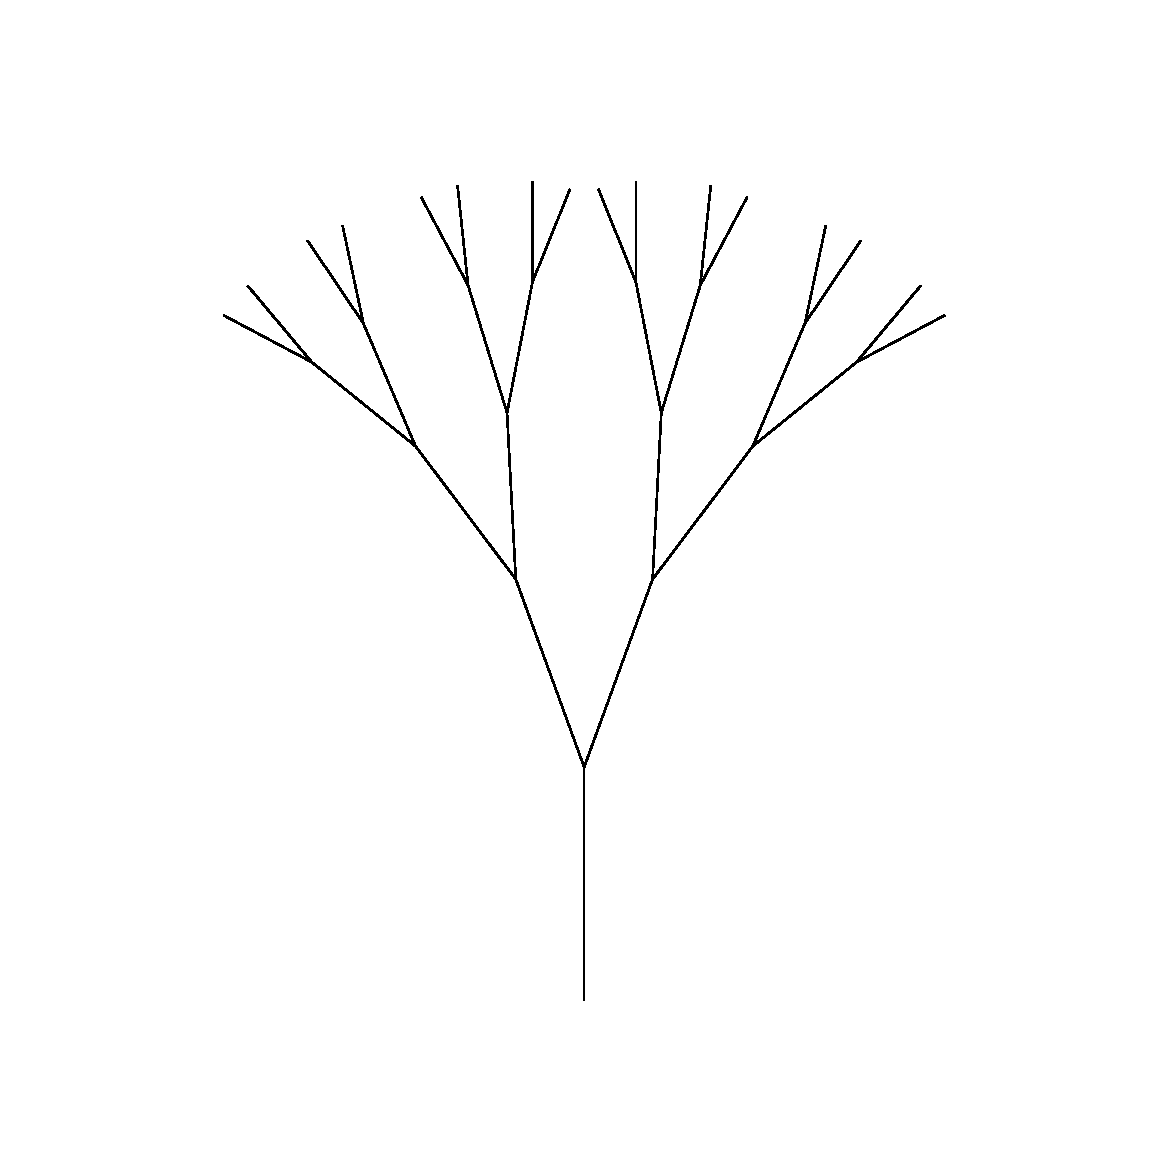
\includegraphics[width=\textwidth]{krunimir/examples/bintree}
    \caption{Binární strom}\label{fig:krunimir-bintree}
  \end{subfigure}

  \caption{Výsledné obrázky z příkladů}
  \label{fig:krunimir-examples}
\end{figure}

\section{Analýza}

Problém si můžeme rozdělit na tři části:

\begin{enumerate}

\item \emph{Syntaktická analýza} (\uv{parsování}) zpracuje vstupní řetězec na
  \emph{abstraktní syntaktický strom}, který zachycuje strukturu programu ve
  formě, která je jednoduše zpracovatelná v dalších fázích.

\item Následuje \emph{vyhodnocení}, kdy ze syntaktického stromu vypočteme
  výslednou stopu (ve vektorové podobě jako seznam úseček).

\item Poslední částí je \emph{vykreslení}, které vykreslí vyhodnocenou stopu do
  obrázku. Budeme exportovat do rastrových obrázků formátu PNG a vektorových
  formátu SVG.

\end{enumerate}

Pomocí tohoto jednoduchého rozdělení můžeme naše řešení rozvrhnout do sedmi
modulů:

\begin{description}

\item @t{Krunimir.Main} exportuje @t{main}, která slouží jako rozhraní s
uživatelem.\footnote{Podobně jako funkce @t{main()} v jazyku C}
  @idx{Krunimir.Main}
  @idx{Krunimir.Main.main}

\item @t{Krunimir.Parser} exportuje funkci @t{parse}, která z textového
zápisu programu vytvoří syntaktický strom (nebo syntaktickou chybu, pokud
program není korektní).
  @idx{Krunimir.Parser}
  @idx{Krunimir.Parser.parse}

\item @t{Krunimir.Ast} definuje datové typy, které reprezentují syntaktický
strom.
  @idx{Krunimir.Ast}

\item @t{Krunimir.Evaluator} poskytuje funkci @t{eval}, která ze
syntaktického stromu vypočte výslednou stopu.
  @idx{Krunimir.Evaluator}
  @idx{Krunimir.Evaluator.eval}

\item @t{Krunimir.Trace} definuje datové typy a funkce spojené se stopou želvy.
  @idx{Krunimir.Trace}

\item @t{Krunimir.PngRenderer} exportuje funkci @t{renderPng}, která vykreslí
  stopu jako PNG obrázek.
  @idx{Krunimir.PngRenderer}
  @idx{Krunimir.PngRenderer.renderPng}

\item @t{Krunimir.SvgRenderer} poskytuje funkci @t{renderSvg}, jenž uloží stopu
  ve vektorovém formátu SVG.
  @idx{Krunimir.SvgRenderer}
  @idx{Krunimir.SvgRenderer.renderSvg}

\end{description}

\input{krunimir/Krunimir/Main.lhs}
\input{krunimir/Krunimir/Ast.lhs}
\input{krunimir/Krunimir/Parser.lhs}
\input{krunimir/Krunimir/Trace.lhs}
\input{krunimir/Krunimir/Evaluator.lhs}
\input{krunimir/Krunimir/PngRenderer.lhs}
\input{krunimir/Krunimir/SvgRenderer.lhs}

\section{Příklady}

Závěrem uvedeme několik rozsáhlejších příkladů, kdy využijeme želví grafiku k
vykreslení několika známých fraktálů. 

\subsection{Hilbertova křivka}

Hilbertova křivka je plochu vyplňující fraktál popsaný roku 1891 německým
matematikem Davidem Hilbertem. \cite{wiki:hilbert-curve} První čtyři iterace
této křivky jsou zakresleny na obrázku \ref{fig:krunimir-hilbert-gen}.

Hlavní část programu je procedura @t{hilbert(n,side)}, která nakreslí Hilbertovu
křivku @t{n}-té iterace. Parametr @t{side} nabývá hodnot @t{-1} a @t{1} a
určuje, na kterou stranu se křivka nakreslí. Výsledek programu je na obrázku
\ref{fig:krunimir-hilbert}.

\lstinputlisting[style=krunimir]{krunimir/examples/hilbert.txt}

\begin{figure}
  \centering
  \caption{Hilbertova křivka}
  \label{fig:krunimir-hilbert-all}

  \begin{subfigure}{0.8\textwidth}
    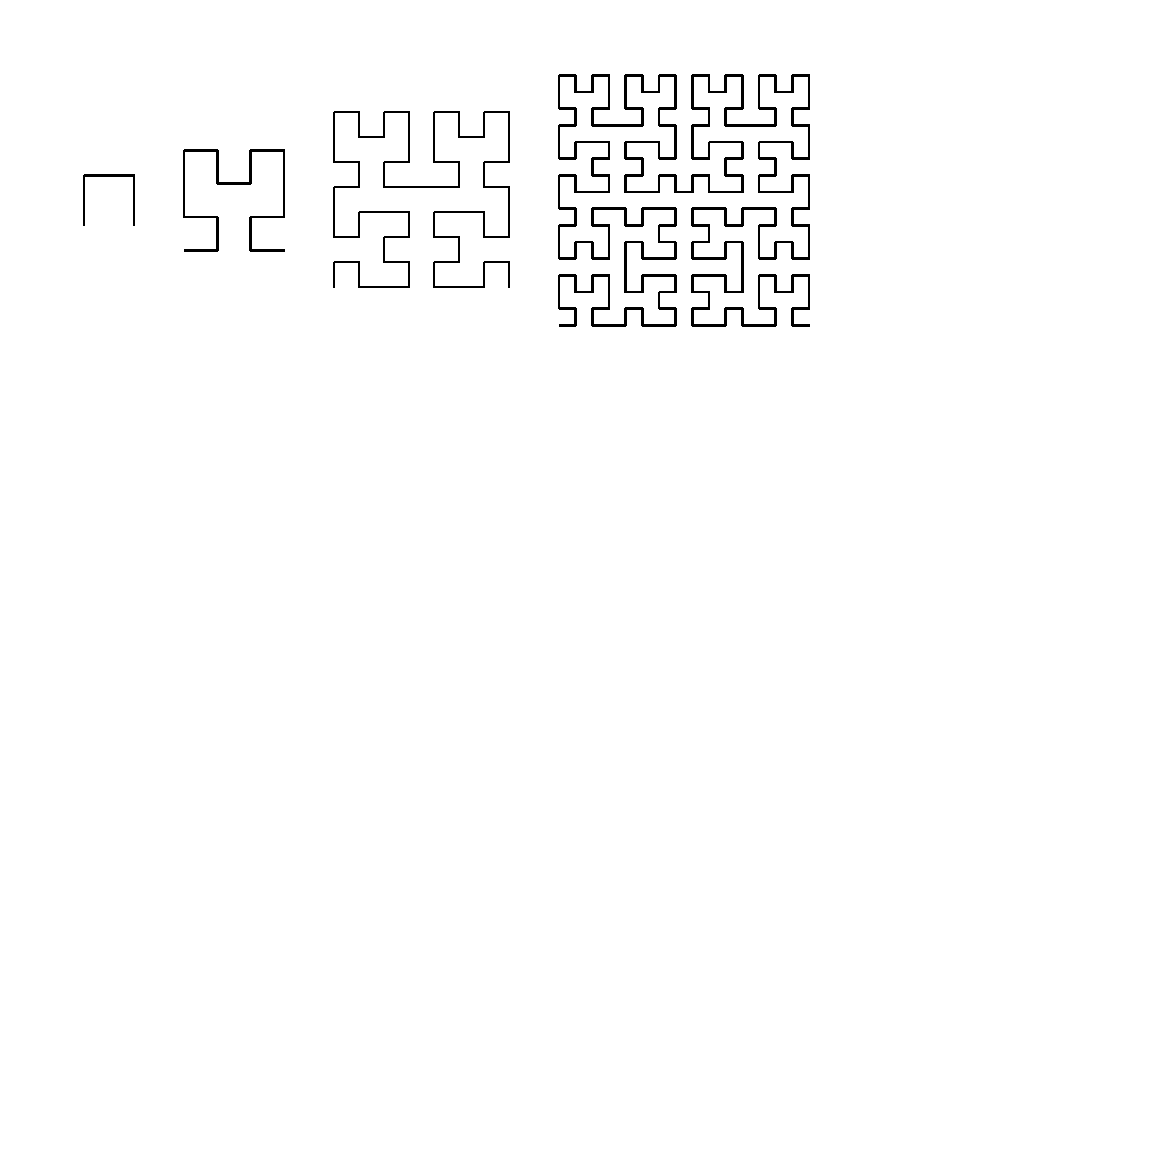
\includegraphics[width=\textwidth,trim=0 400 150 0]{krunimir/examples/hilbert-gen}
    \caption{Postupné generování Hilbertovy křivky (zleva doprava iterace 1 až 4).}
    \label{fig:krunimir-hilbert-gen}
  \end{subfigure}

  \begin{subfigure}{0.8\textwidth}
    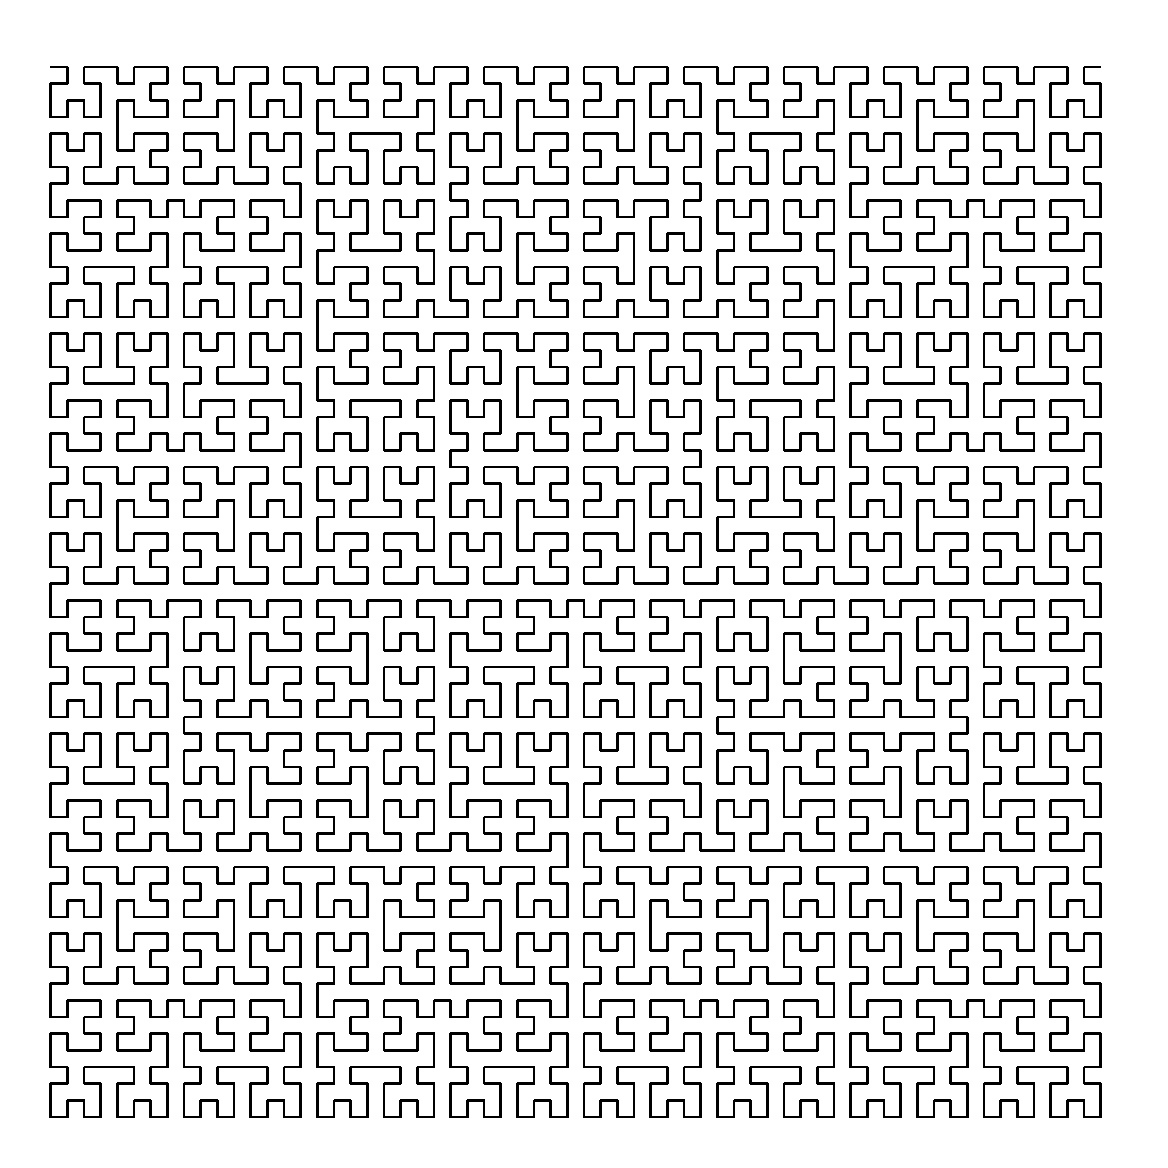
\includegraphics[width=\textwidth]{krunimir/examples/hilbert}
    \caption{Hilbertova křivka vykreslená Krunimírem}
    \label{fig:krunimir-hilbert}
  \end{subfigure}
\end{figure}

\subsection{Kochova vločka}

Kochova vločka je známý fraktál založený na Kochově křivce, kterou v roce 1904
vytvořil švédský matematik Helge von Koch. \cite{wiki:koch-snowflake}

Obrázek \ref{fig:krunimir-koch-gen} zachycuje první čtyři iterace Kochovy
křivky. O kreslení se stará procedura @t{koch(n)}, jež nakreslí @t{n}-tou
iteraci Kochovy křivky. Tuto proceduru posléze zavoláme třikrát po sobě, čímž
vytvoříme Kochovu vločku. Výsledek programu je na obrázku
\ref{fig:krunimir-koch}.

\lstinputlisting[style=krunimir]{krunimir/examples/koch.txt}

\begin{figure}
  \centering
  \caption{Kochova vločka}
  \label{fig:krunimir-koch-all}

  \begin{subfigure}{0.8\textwidth}
    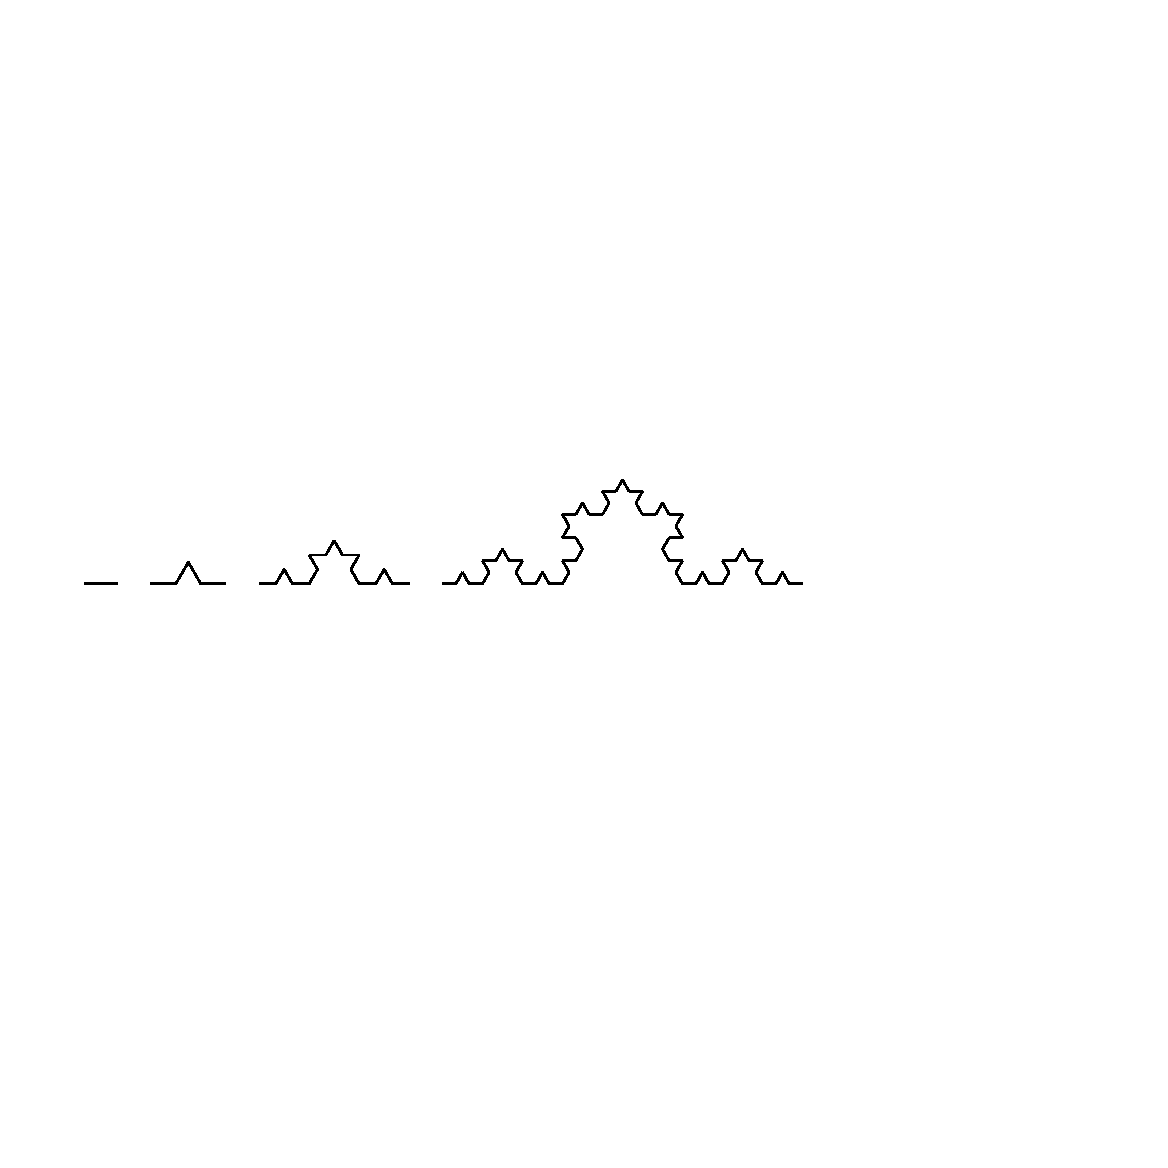
\includegraphics[width=\textwidth,trim=0 250 150 200]{krunimir/examples/koch-gen}
    \caption{Iterace Kochovy křivky. Kochovu vločku dostaneme spojením
    tří Kochových křivek.}
    \label{fig:krunimir-koch-gen}
  \end{subfigure}

  \begin{subfigure}{0.9\textwidth}
    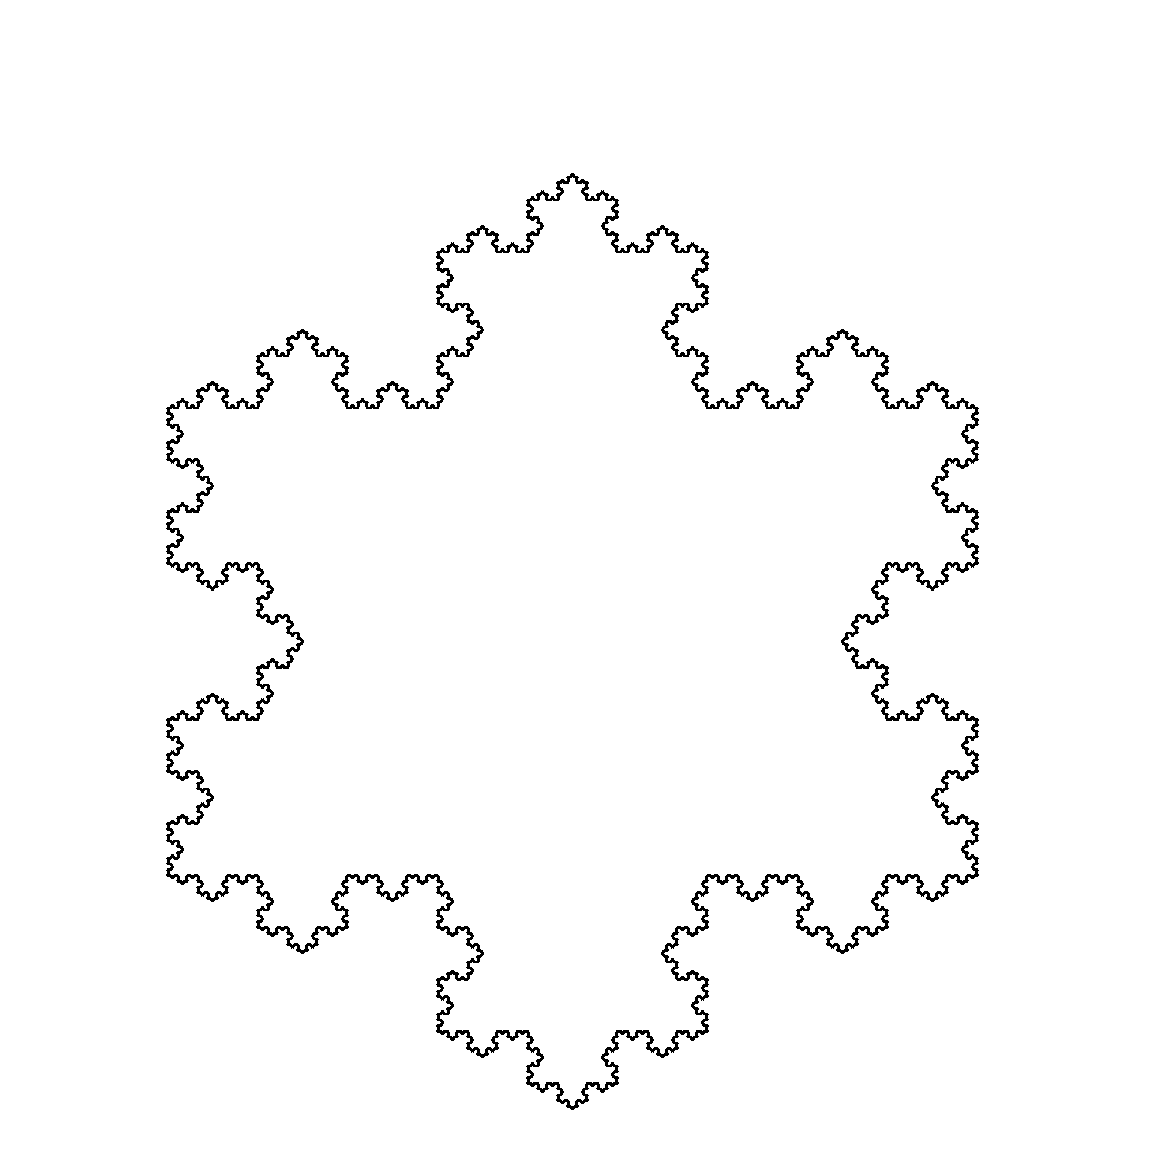
\includegraphics[width=\textwidth]{krunimir/examples/koch}
    \caption{Kochova vločka vykreslená Krunimírem}
    \label{fig:krunimir-koch}
  \end{subfigure}
\end{figure}

\subsection{Gosperova křivka}

Gosperova křivka, pojmenovaná po svém objeviteli, americkém programátorovi a
matematikovi Billu Gosperovi, je plochu vyplňující fraktál.
\cite{wiki:gosper-curve}

Na vykreslení této křivky musíme použít dvojici procedur, @t{gosperA} a
@t{gosperB}, přičemž každá kreslí křivku z jiné strany (odpředu a odzadu).
Způsob generování je zobrazen na obrázku \ref{fig:krunimir-gosper-gen}, výstup
programu na obrázku \ref{fig:krunimir-gosper}.

\lstinputlisting[style=krunimir]{krunimir/examples/gosper.txt}

\begin{figure}
  \centering
  \caption{Gosperova křivka}
  \label{fig:krunimir-gosper-all}

  \begin{subfigure}{0.8\textwidth}
    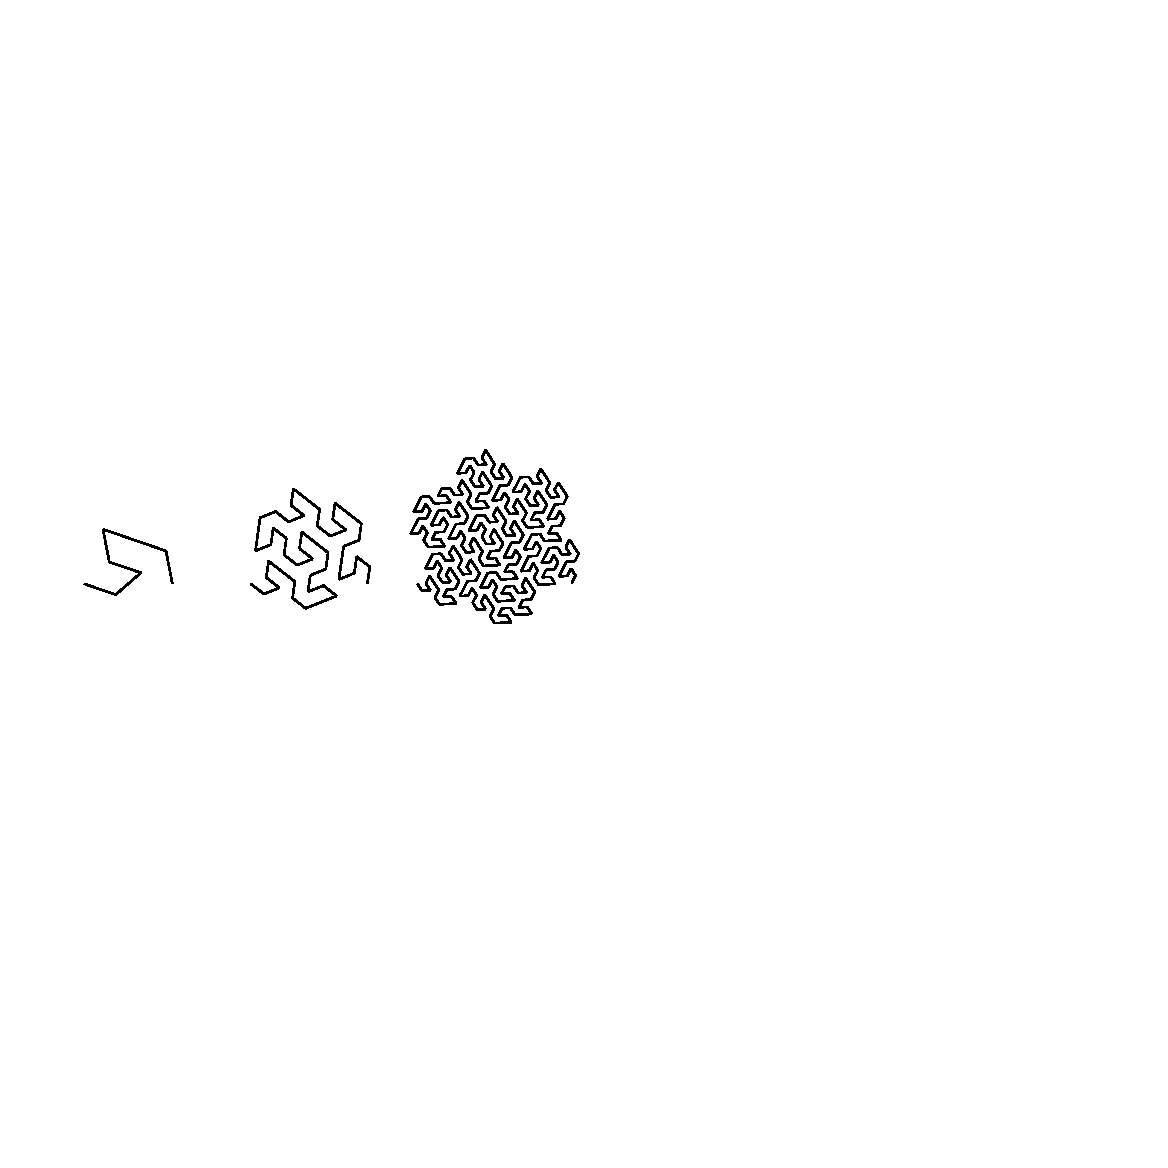
\includegraphics[width=\textwidth,trim=0 250 250 200]{krunimir/examples/gosper-gen}
    \caption{První tři iterace Gosperovy křivky.}
    \label{fig:krunimir-gosper-gen}
  \end{subfigure}

  \begin{subfigure}{0.9\textwidth}
    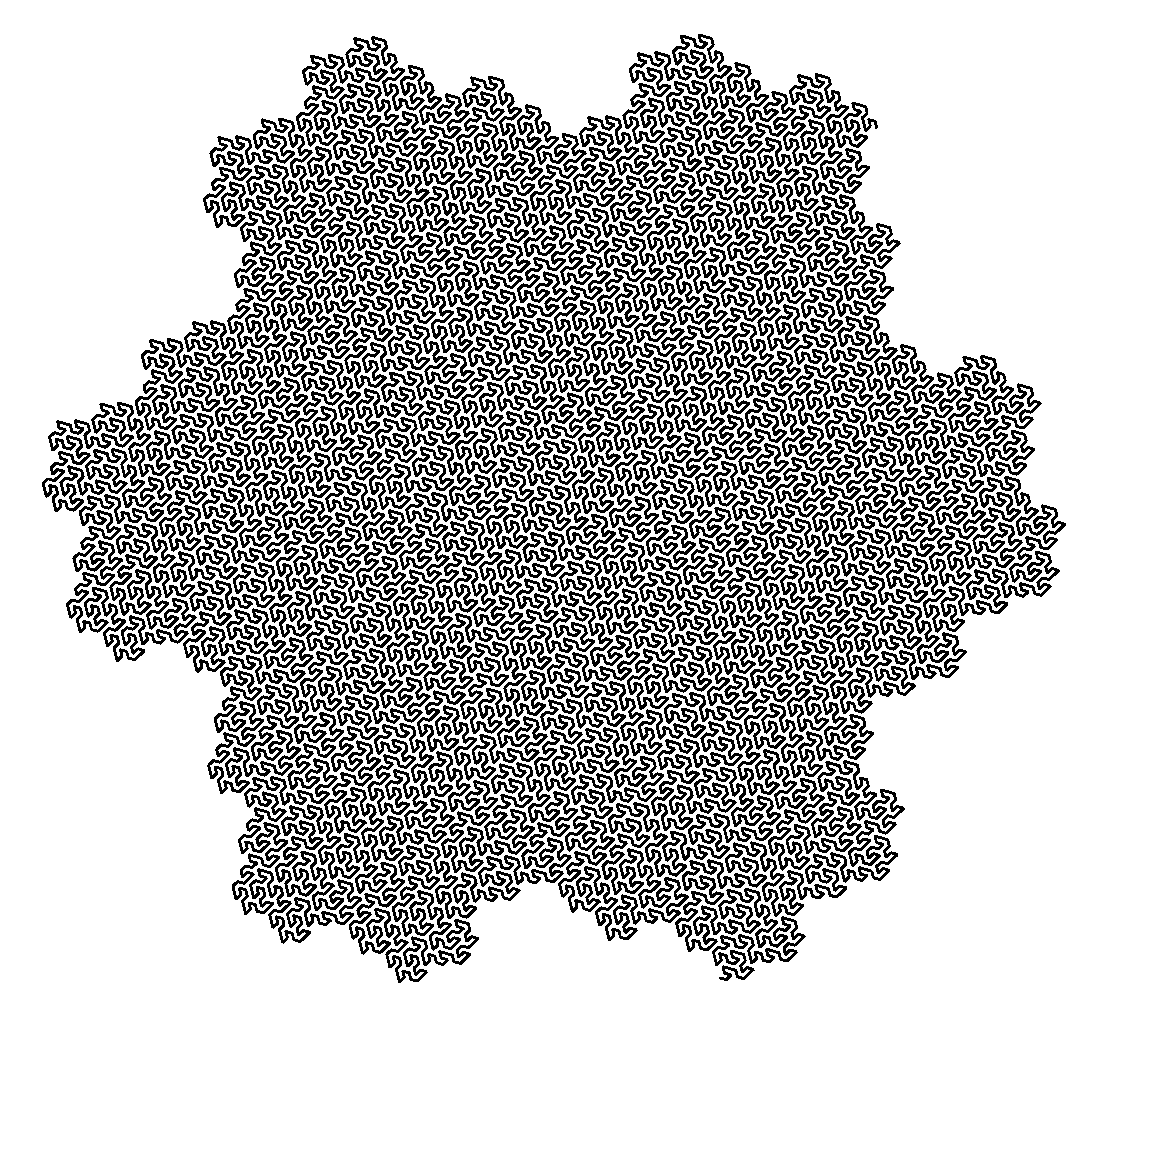
\includegraphics[width=\textwidth]{krunimir/examples/gosper}
    \caption{Gosperova křivka vykreslená Krunimírem}
    \label{fig:krunimir-gosper}
  \end{subfigure}
\end{figure}

\subsection{Křivka arrowhead}

Křivka arrowhead je podobná Sierpi\`nského trojúhelníku, fraktálu polského
matematika Wac\l{}ava Sierpi\`nského, který jej popsal v roce 1915.
\cite{wiki:arrowhead-curve}

Podobně jako u Hilbertovy křivky i zde musíme počítat s tím, že křivku musíme
vykreslovat ve dvou zrcadlových variantách, k čemuž využijeme parametr @t{side}
procedury @t{arrowhead(n,side)}. Postup generování ukazuje obrázek
\ref{fig:krunimir-arrowhead-gen}, výsledek programu obrázek
\ref{fig:krunimir-arrowhead}.

\lstinputlisting[style=krunimir]{krunimir/examples/arrowhead.txt}

\begin{figure}
  \centering
  \caption{Křivka arrowhead}
  \label{fig:krunimir-arrowhead-all}

  \begin{subfigure}{0.8\textwidth}
    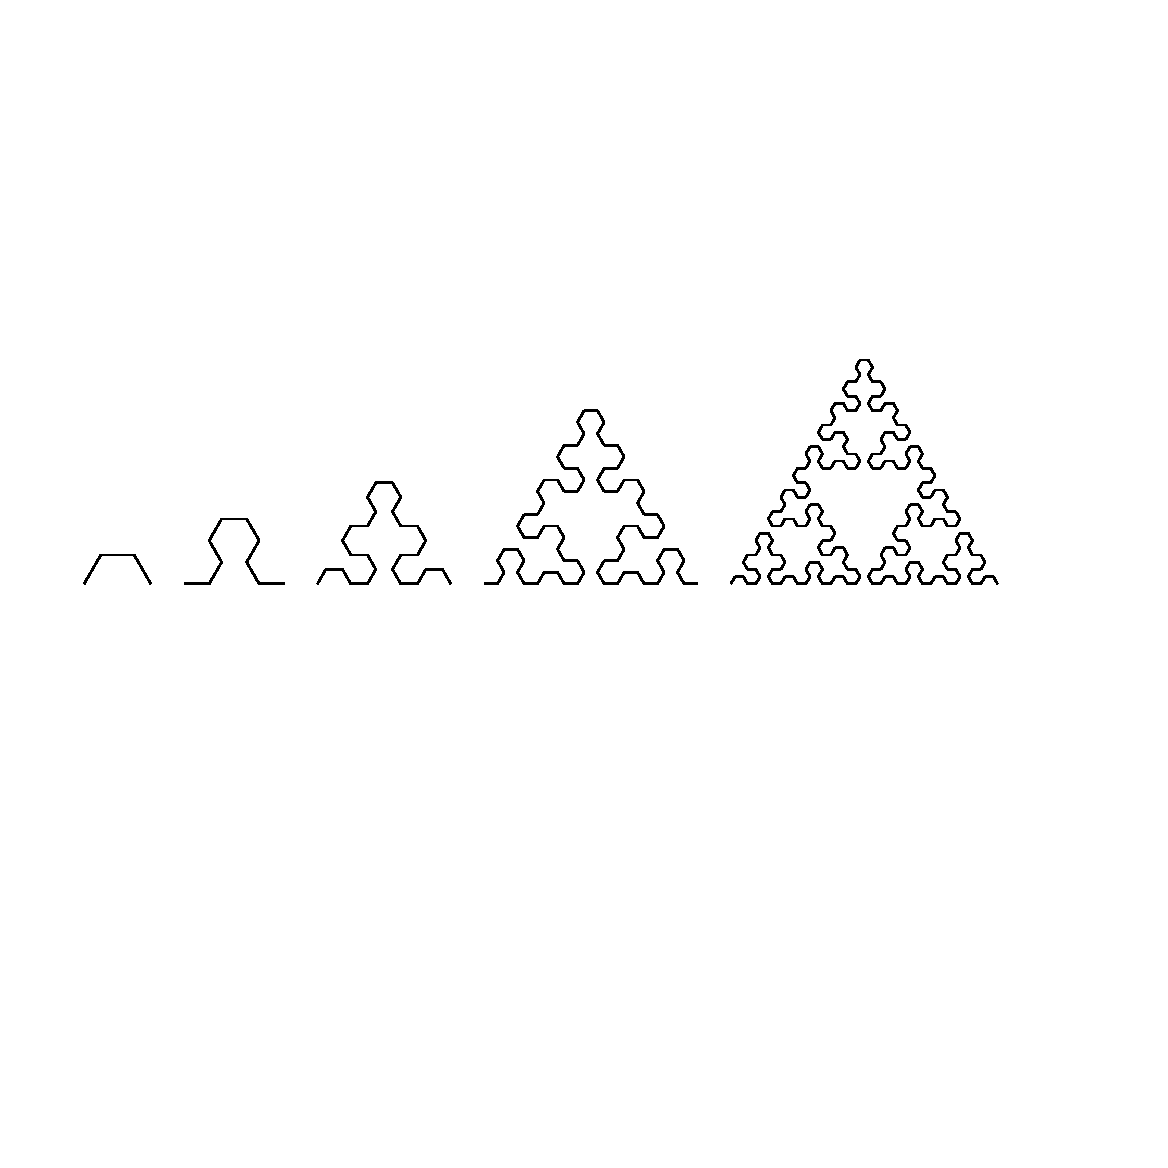
\includegraphics[width=\textwidth,trim=0 250 50 150]
      {krunimir/examples/arrowhead-gen}
    \caption{Prvních pět iterací křivky arrowhead.}
    \label{fig:krunimir-arrowhead-gen}
  \end{subfigure}

  \begin{subfigure}{0.9\textwidth}
    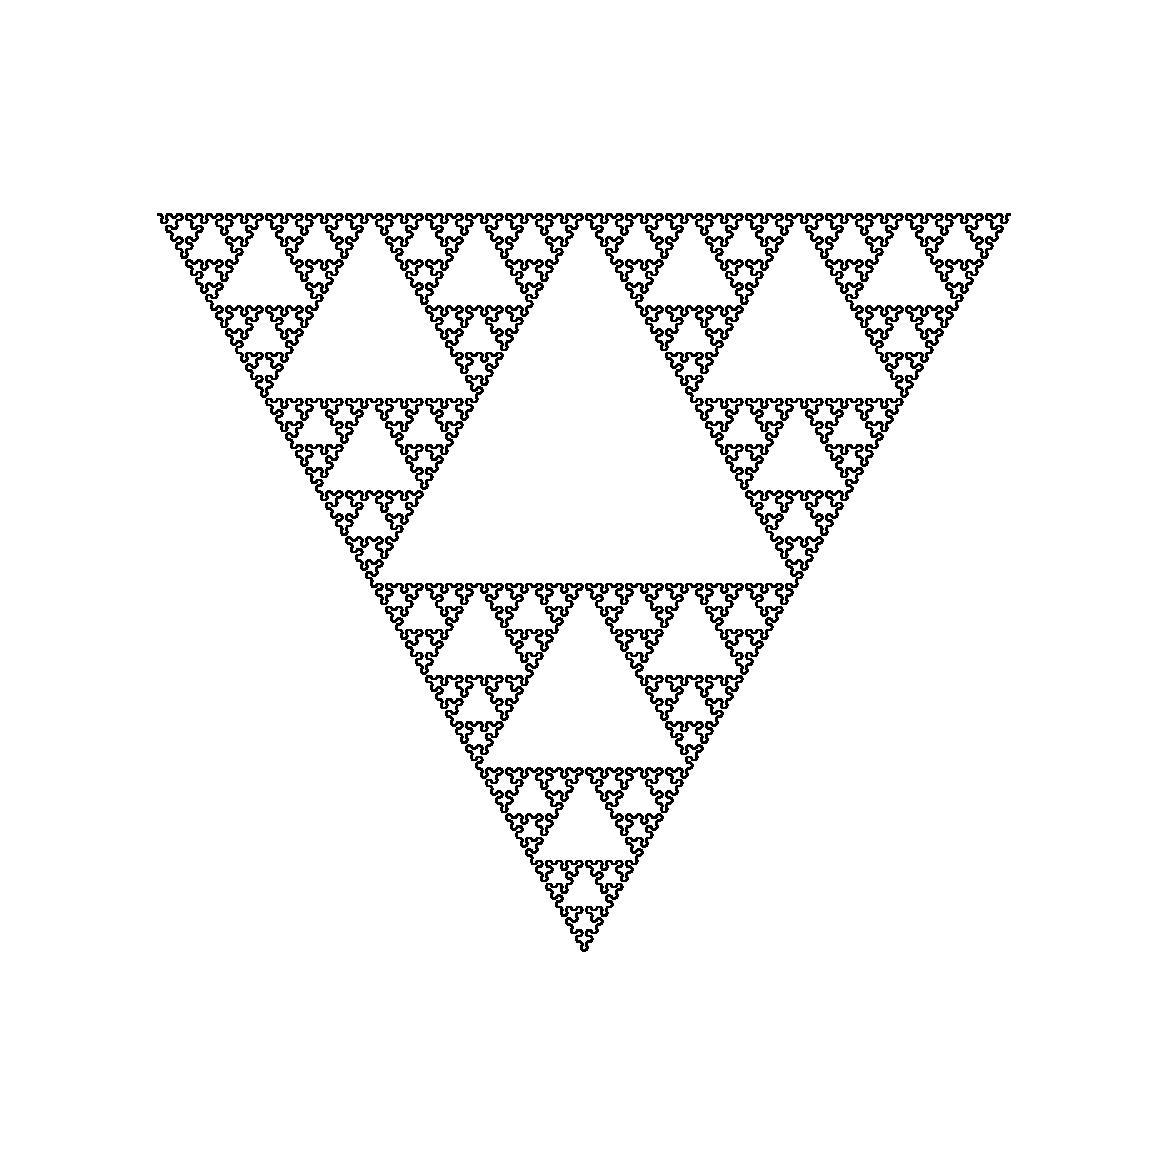
\includegraphics[width=\textwidth]{krunimir/examples/arrowhead}
    \caption{Křivka arrowhead vykreslená Krunmírem}
    \label{fig:krunimir-arrowhead}
  \end{subfigure}
\end{figure}

\section{Závěr}

Vytvořili jsme interpret zadaného programovacího jazyka Krunimír, podporující
veškerá rozšíření, vykreslování do dvou grafických formátů, a s velmi
přijatelným výkonem.

Představený program by byl podle zadání ze soutěže nejspíše ohodnocen přibližně
300 body z 333.  Chybějících 33 bodů je za \uv{televizní přenos}, neboli
grafické uživatelské rozhraní (GUI). Tvorba GUI není nijak zvlášť
programátorsky zajímavá, proto ji náš program neimplementuje.

Všechny zdrojové soubory mají dohromady asi 350 řádků kódu. Vezmeme-li v úvahu,
že se jedná o kompletní implementaci netriviálního programovacího jazyka, je
toto číslo poměrně nízké.\footnote{Je nutno podotknout, že program nebyl psán
  tak, aby řádků bylo co nejméně, ale aby byl co nejpřehlednější.} Kód je
rozdělen do modulů s minimálními vzájemnými závislostmi, může tedy být snadno
udržován, upravován a rozšiřován.

Pokud bychom namísto Haskellu použili nějaký imperativní programovací jazyk,
například \Cplusplus{}, Ruby\footnote{
  Pokud bychom využili dynamický jazyk jako
  Ruby, mohli bychom si ušetřit práci a několika jednoduchými textovými úpravami
  převést program pro Krunimíra na program v použitém programovacím jazyku,
  který bychom vyhodnotili pomocí funkce @t{eval}. Tento postup svého času autor
  na soutěži úspěšně využil.  Jedinou nevýhodou je nesnadnost korektní
  implementace příkazu @t{split}, jinak jde o řešení téměř dokonalé :-) 
} nebo dokonce Javu, náš program by byl nejspíš delší a jeho modularita by byla
nižší. Program by pravděpodobně sestával z parseru vytvořeného pomocí nějakého
externího nástroje, který by vytvořil syntaktický strom sestávající z objektů.
Vyhodnocení by bylo sloučeno s vykreslováním a probíhalo by voláním metod
objektů ze syntaktického stromu, jejichž definice by byly roztroušeny u definic
jednotlivých tříd.\footnote{
  V Javě bychom nejspíše vytvořili třídu @t{Statement}, která by měla potomky
  @t{ForwardStatement}, @t{LeftStatement}, @t{RepeatStatement} apod. přičemž
  každý by byl ve vlastním souboru...  
  } Implementovat příkaz @t{split} by bylo přinejmenším obtížné.

\subsection{Zdrojové kódy}

Veškeré soubory související s Krunimírem jsou v repozitáři s prací uloženy
ve složce @t{krunimir/}. Zdrojové kódy všech uvedených modulů jsou ve složce
@t{krunimir/Krunimir}, testovací soubory ve složce @t{krunimir/test}. Část
testovacích souborů pochází ze soutěže, část byla vytvořena v rámci této práce.

Pro testování je možné použít skript @t{runtest.sh}, který spustí program pro
všechny soubory ze složky @t{krunimir/test}. Výsledné soubory (s příponou
@t{.test.png} a @t{.test.svg}) je pak možno vizuálně porovnat s očekávanými
výsledky (přípona pouze @t{.png}).

Složka @t{krunimir/examples} obsahuje zdrojové kódy příkladů, ze kterých se
generují obrázky, jež jsou v práci vloženy.
